We now turn to a completely different meaning of \textit{multiobjective}. Let us take a few steps back. Throughout this book, we have studied two types of interaction between players: rational, antagonistic interaction between Eve and Adam; and stochastic interaction with a random player. Consider the quantitative settings of~\cref{chap:payoffs} and~\cref{chap:mdp}. In the zero-sum two-player games of the former, Adam is seen as a \textit{purely antagonistic adversary}, so the goal of Eve is to ensure strict ""worst-case guarantees"", i.e., a minimal performance level against all possible strategies of Adam. In the MDPs of the latter, Eve interacts with randomness (through actions or random vertices) and she wants to ensure a good \textit{"expected value"} for the considered payoff.

For most objectives, these two paradigms yield elegant and simple solutions: e.g., memoryless strategies suffice for both games and MDPs with a mean-payoff objective. Nevertheless, the corresponding strategies have clear weaknesses: strategies that are good for the worst-case may exhibit suboptimal behaviours in probable situations while strategies that are good for the expected value may be terrible in some unlikely but possible situations. A natural question, of theoretical and practical interest, is to build -- \textit{synthesize} -- strategies that combine both paradigms: strategies that both ensure (a) some worst-case threshold no matter how the adversary behaves (i.e., against any arbitrary strategy) and (b) a good expectation against the expected behaviour of the adversary (given as a stochastic model). We call this task ""beyond worst-case synthesis"".

The goal of this section is to illustrate the complexity of beyond worst-case synthesis and how it requires fine-tuned interaction between the worst-case and average-case aspects. To that end, we focus on a specific case: the synthesis of \textit{finite-memory strategies} for beyond worst-case \textit{mean-payoff} objectives. Due to the highly technical nature of this approach, we will not present all its details, but rather paint in broad strokes its cornerstones. We hope to give the reader sufficient intuition and understanding to develop a clear view of the challenges arising from rich behavioural models, and some of the techniques that come to the rescue. 

\subsection{The decision problem}

Our goal is to mix the games of~\cref{chap:payoffs} and the MDPs of~\cref{chap:mdp}, so we need to go back and forth between these models.

\paragraph{Two-player game} As before, we start with an arena $\arena = (G = (V, E), V_{\text{Eve}}, V_{\text{Adam}})$, where the vertices are split between Eve's and Adam's. This arena represents the antagonistic interaction between Eve and Adam, so we consider a worst-case constraint on the corresponding game. We study a single mean-payoff function, so our colouring is $c\colon E \to \Z$. Let $\alpha \in \Q$ be the worst-case threshold: we are looking for a strategy of Eve that is winning for objective $\MeanPayoff^{-}_{> \alpha}$. Two things to note: first, we consider the lim-inf variant w.l.o.g.~as we focus on \textit{finite-memory} strategies (recall~\cref{12-prop:MPSI}); second, we use a strict inequality as it will ease the formulation of the upcoming results.

\paragraph{MDP} To make the connection with MDPs, we fix a finite-memory randomized strategy for Adam in the arena $\arena$, $\tau^\text{stoch}$. Recall that a randomized strategy \todo{It seems this is never addressed properly before but used in MDPs, stochastic games, etc: to sort out before its first use.} is a function $E^* \to \mathcal{D}(E)$. As usual, we may build $\arena_{\tau^\text{stoch}}$, the product of the arena $\arena$ with the memory structure of $\tau^\text{stoch}$, restricted to the choices made by $\tau^\text{stoch}$. Since $\tau^\text{stoch}$ is assumed to be stochastic, what we obtain is not a one-player game for Eve, but an MDP.

To understand this relationship, it is easier to consider the alternative -- and equivalent -- formalism of MDPs, based on random vertices (as used for stochastic games in~\cref{chap:stochastic}). Assume for instance that $\tau^\text{stoch}$ is a randomized memoryless strategy, i.e., a function $V_{\Adam} \to \mathcal{D}(E)$. Then, the MDP $\arena_{\tau^\text{stoch}}$ is immediately obtained by replacing each Adam's vertex $v$ by a random vertex such that $\delta(v) = \tau^\text{stoch}(v)$, i.e., the probabilistic transition function uses the same probability distributions as Adam's strategy. Formally, we build the MDP $\mathcal{P} = \arena_{\tau^{\text{stoch}}} = (G, V_{\text{Eve}}, V_{\text{Rand}} = V_{\text{Adam}}, \delta = \tau^{\text{stoch}})$.

In contrast to~\cref{chap:stochastic}, we explicitly allow the transition function to assign probability zero to some edges of the underlying graph $G$, i.e., the support of $\delta(v)$ in some vertex $v \in V_{\text{Rand}}$ might not include all edges $e \in E$ such that $\ing(e) = v$.
This is important as far as modelling is concerned, as in our context, transition functions will be defined according to a stochastic model for Adam, and we cannot reasonably assume that such a model always involves all the possible actions of Adam. Consequently, given the MDP $\markovProcess$, we define the subset of edges $\edgesNonZero = \{ e \in E \mid \ing(e) \in V_{\text{Rand}} \implies \delta(\ing(e))(e) > 0\}$, representing all edges that either start in a vertex of Eve, or are chosen with non-zero probability by the transition function $\delta$. Edges in $E\setminus \edgesNonZero$ will only matter in the two-player game interpretation, whereas all MDP-related concepts, such as "end-components", are defined with regard to edges in $\edgesNonZero$ exclusively.

\paragraph{Beyond worst-case problem} Let us sum up the situation: we have a two-player arena $\arena$ with a mean-payoff objective $\MeanPayoff^{-}_{> \alpha}$ and a finite-memory stochastic model for Adam yielding the MDP $\arena_{\tau^\text{stoch}}$. Now, let $\beta \in \Q$ be the expected value threshold we want to ensure in the MDP (i.e., on average against the stochastic model of Adam).


\decpb{Beyond worst-case}{An arena $\arena$, a finite-memory stochastic model $\tau^\text{stoch}$, an\\ & initial vertex $v_0$, two thresholds $\alpha, \beta \in \Q$\\}{Does Eve have a \textit{finite-memory} strategy $\sigma$ such that $\sigma$ is \\ & winning for objective $\MeanPayoff^{-}_{> \alpha} \text{ from } v_0 \text{ in } \arena$\\ &
and $\expv^{\sigma}_{\arena_{\tau^\text{stoch}},v_0}[\MeanPayoff^{-}] > \beta$?}

We assume $\beta > \alpha$, otherwise the problem trivially reduces to the classical worst-case analysis: if all plays consistent with $\sigma$ have mean-payoff greater than $\alpha \geq \beta$ then the expected value is also greater than $\alpha$ regardless of the stochastic model.

\subsection{The approach in a nutshell}
We present our solution to the BWC problem in~\cref{12-algo:BWC}. We give an intuitive sketch of its functioning in the following, and illustrate it on a toy example. 

DO SOMETHING WITH THIS ALGORITHM IT DOES NOT COMPILE!!!
%\begin{algorithm}[thb]
% \KwData{Arena $\arena^i = (G^i = (V^i, E^i), V^i_{\text{Eve}}, V^i_{\text{Adam}})$, colouring $c^i\colon E \to \Z$, finite-memory stochastic model $\tau^i$ for Adam with memory structure $\mem$ and initial memory state $m_0$, worst-case and expected value thresholds $\alpha^i = a/b, \beta^i \in \Q$, $\alpha^i < \beta^i$, initial vertex $v^i_0 \in V^i$}
% \KwResult{\textsc{Yes} if and only if Eve has a finite-memory strategy $\sigma$ for the BWC problem from $v^i_0$ for thresholds pair $(\alpha^i, \beta^i)$}
% \tcc{Preprocessing}
% \If{$\alpha^i \neq 0$}{
% 	Modify the colouring: $\forall e \in E^i$, $c(e) \leftarrow b\cdot c^i(e) - a$\;
% 	Consider the new thresholds pair $(0, \beta \leftarrow b\cdot \beta^i - a)$\;
% }
% \Else{
% 	$c \rightarrow c^i$
% }
% $V_{\text{WC}} \leftarrow \textsf{SolveWorstCaseMeanPayoff}(\arena, c)$\;
% \If{$v^i_0 \not\in V_{\text{WC}}$}{
% 	\Return \textsc{No}
% }
% \Else{
%    $\arena^{w} \leftarrow \arena^i \downharpoonright V_{\text{WC}}$\tcc*{Restriction of $\arena^i$ to $V_{\text{WC}}$}
% 	Let $\arena \leftarrow \arena^{w} \times \mem = (G = (V, E), V_{\text{Eve}}, V_{\text{Adam}})$ be the arena obtained by product with the memory structure of Adam's stochastic model $\tau^i$\;
% 	Let $v_0 \leftarrow (v^i_0, m_0)$ be the corresponding initial vertex in $\arena$\;
% 	Let $\tau^{\text{stoch}}$ be the memoryless transcription of $\tau^i$ on $\arena$\;
% 	Let $\mathcal{P} \leftarrow \arena_{\tau^{\text{stoch}}} = (G, V_{\text{Eve}}, V_{\text{Rand}} = V_{\text{Adam}}, \delta = \tau^{\text{stoch}})$ be the corresponding MDP\tcc*{Random vertices formalism}
% }
% \tcc{Main algorithm}
% Compute $\mathcal{U}_{W}$ the set of \textit{maximal winning end-components} of $\mathcal{P}$\;
% Modify the colouring:\begin{equation*}
%\forall\, e \in E,\, c'(e) \leftarrow \begin{cases}c(e) \text{ if } \exists\: U \in \mathcal{U}_{W} \text{ s.t. } \{\ing(e), \out(e)\} \subseteq U\\0 \text{ otherwise} \end{cases}
%\end{equation*}\\
%Compute the maximal expected value $\beta^\ast$ from $v_0$ in $\mathcal{P}$ using $c'$\;
%\If{$\beta^\ast > \beta$}{
%	\Return \textsc{Yes}
%}
%\Else{
%	\Return \textsc{No}
%}
%\caption{Solver for the beyond worst-case mean-payoff problem}
%\label{12-algo:BWC}
%\end{algorithm}


\subsection*{Inputs and outputs} The algorithm takes as input: an arena $\arena^{i}$, a finite-memory stochastic model of Adam $\tau^{i}$, a worst-case threshold $\alpha^{i}$, an expected value threshold $\beta^{i}$, and an initial vertex $v_0^{i}$. Its output is $\textsc{Yes}$ if and only if there exists a finite-memory strategy of Eve satisfying the BWC problem.

The output as described in~\cref{12-algo:BWC} is Boolean: the algorithm answers whether a satisfying strategy exists or not, but does not explicitly construct it (to avoid tedious formalization within the pseudocode). Nevertheless, we sketch the synthesis process in the following and we highlight the role of each step of the algorithm in the construction of a winning strategy, as producing a witness winning strategy is a straightforward by-product of the process we apply to decide satisfaction of the BWC problem.


\subsection*{Preprocessing} The first part of the algorithm is dedicated to the preprocessing of the arena $\arena^{i}$ and the stochatic model $\tau^{i}$ given as inputs in order to apply the second part of the algorithm on a modified arena $\arena$ and stochastic model $\tau^{\text{stoch}}$, simpler to manipulate. We show in the following that the answer to the BWC problem on the modified arena is $\textsc{Yes}$ if and only if it is also $\textsc{Yes}$ on the input arena, and we present how a winning strategy of Eve in $\arena$ can be transferred to a winning strategy in $\arena^{i}$.

The preprocessing is composed of four main steps. First, we modify the colouring function $c^i$ in order to consider the equivalent BWC problem with thresholds $(0,\, \beta)$ instead of $(\alpha^{i},\, \beta^{i})$. This classical trick is used to get rid of explicitly considering the worst-case threshold in the following, as it is equal to zero.

Second, observe that any strategy that is winning for the BWC problem must also be winning for the classical \textit{worst-case problem}, as solved in the two-player games of~\cref{chap:payoffs}. Such a strategy cannot allow visits of any vertex from which Eve cannot ensure winning against an antagonistic adversary because mean-payoff is a prefix independent objective (hence it is not possible to ``win'' it over the finite prefix up to such a vertex). Thus, we reduce our study to $\arena^{w}$, the subarena induced by Eve's worst-case winning vertices -- which we compute in pseudo-poly\-nomial time thanks to $\textsf{SolveWorstCaseMeanPayoff}(\arena, c)$ (implementing the algorithm of~\cref{chap:payoffs}). \todo{I need a label on Subsect. 4.3.4 to cite it precisely.}  Note that we use the modified colouring and that $\arena^{w}$ is a proper arena (same argument as~\cref{12-rmk:properArena}). Obviously, if from the initial vertex $v_0^{i}$, Eve cannot win the worst-case problem, then the answer to the BWC problem is \textsc{No}.

Third, we build arena $\arena$, the product of $\arena^{w}$ and the memory structure of Adam's stochastic model $\tau^i$. Intuitively, we expand the initial arena by integrating the memory elements in the graph. Note that this does not modify the power of Adam in the two-player interpretation of the arena.

Fourth, the finite-memory stochastic model $\tau^{i}$ on $\arena^{i}$ clearly translates to a memoryless stochastic model $\tau^{\text{stoch}}$ on $\arena$. This will help us obtain elegant proofs for the second part of the algorithm.

\begin{example}
\begin{figure}[tbh]
  \centering   
  \scalebox{0.8}{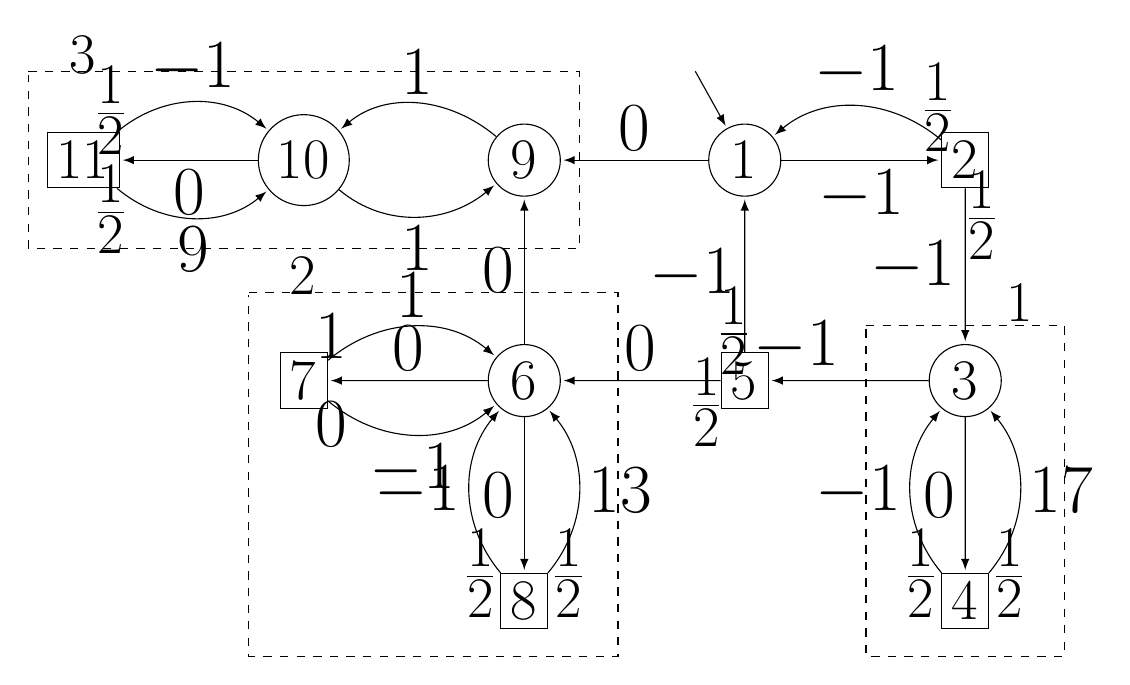
\begin{tikzpicture}[->,>=latex,shorten >=1pt,auto,node
    distance=2.5cm,bend angle=45,font=\Huge,scale=0.7]
    \tikzstyle{p1}=[draw,circle,text centered,minimum size=6mm]
    \tikzstyle{p2}=[draw,rectangle,text centered,minimum size=6mm]
    \tikzstyle{empty}=[]
    \node[p1] (1) at (0,0) {$\state_{9}$};
    \node[p1] (2) at (4,0) {$\state_{1}$};
    \node[p2] (3) at (8,0) {$\state_{2}$};
    \node[p1] (4) at (8,-4) {$\state_{3}$};
    \node[p2] (5) at (8,-8) {$\state_{4}$};
    \node[p2] (6) at (4,-4) {$\state_{5}$};
    \node[p1] (7) at (0,-4) {$\state_{6}$};
    \node[p2] (8) at (-4,-4) {$\state_{7}$};
    \node[p1] (9) at (-4,0) {$\state_{10}$};
    \node[p2] (10) at (-8,0) {$\state_{11}$};
    \node[p2] (11) at (0,-8) {$\state_{8}$};
    \node[empty] (swec) at (-8, 1.9) {$\ec_{3}$};
    \node[empty] (wwec) at (-4, -2.1) {$\ec_{2}$};
    \node[empty] (lec) at (9, -2.6) {$\ec_{1}$};
    \node[empty] (proba5a) at (7.2, -7.5) {$\frac{1}{2}$};
    \node[empty] (proba5b) at (8.8, -7.5) {$\frac{1}{2}$};
    \node[empty] (proba3a) at (8.3, -1) {$\frac{1}{2}$};
    \node[empty] (proba3b) at (7.5, 0.95) {$\frac{1}{2}$};
    \node[empty] (proba8a) at (-3.5, -3.2) {$1$};
    \node[empty] (proba8b) at (-3.5, -4.8) {$0$};
    \node[empty] (proba10a) at (-7.5, 0.9) {$\frac{1}{2}$};
    \node[empty] (proba10b) at (-7.5, -0.9) {$\frac{1}{2}$};
    \node[empty] (proba11a) at (0.8, -7.5) {$\frac{1}{2}$};
    \node[empty] (proba11b) at (-0.8, -7.5) {$\frac{1}{2}$};
    \node[empty] (proba6a) at (3.8, -3.1) {$\frac{1}{2}$};
    \node[empty] (proba6b) at (3.3, -4.4) {$\frac{1}{2}$};
    \coordinate[shift={(-3mm,8mm)}] (init) at (2.north west);
    \path
    (2) edge node[above] {$0$} (1)
    (6) edge node[above] {$0$} (7)
    (4) edge node[above left] {$-1$} (6)
    (3) edge node[left] {$-1$} (4)
    (6) edge node[left] {$-1$} (2)
    (4) edge node[left] {$0$} (5)
    (7) edge node[above] {$0$} (8)
    (7) edge node[left] {$0$} (1)
    (init) edge (2)
    ;
	\draw[->,>=latex] (3) to[out=140,in=40] node[above] {$-1$} (2);
	\draw[->,>=latex] (2) to[out=0,in=180] node[below] {$-1$} (3);
	\draw[->,>=latex] (5) to[out=50,in=310] node[right] {$17$} (4);
	\draw[->,>=latex] (5) to[out=130,in=230] node[left] {$-1$} (4);
	\draw[->,>=latex] (8) to[out=40,in=140] node[above] {$1$} (7);
	\draw[->,>=latex] (8) to[out=320,in=220] node[below] {$-1$} (7);
	\draw[->,>=latex] (1) to[out=140,in=40] node[above] {$1$} (9);
	\draw[->,>=latex] (9) to[out=320,in=220] node[below] {$1$} (1);
	\draw[->,>=latex] (9) to[out=180,in=0] node[below] {$0$} (10);
	\draw[->,>=latex] (10) to[out=40,in=140] node[above] {$-1$} (9);
	\draw[->,>=latex] (10) to[out=320,in=220] node[below] {$9$} (9);
	\draw[->,>=latex] (7) to[out=270,in=90] node[left] {$0$} (11);
	\draw[->,>=latex] (11) to[out=130,in=230] node[left] {$-1$} (7);
	\draw[->,>=latex] (11) to[out=50,in=310] node[right] {$13$} (7);
	\draw[dashed,-] (-9,1.6) -- (1,1.6) -- (1,-1.6) -- (-9,-1.6) -- (-9,1.6);
	\draw[dashed,-] (6.2,-3) -- (9.8,-3) -- (9.8,-9) -- (6.2,-9) -- (6.2,-3);
	\draw[dashed,-] (-5,-2.4) -- (1.7,-2.4) -- (1.7,-9) -- (-5,-9) -- (-5,-2.4);
      \end{tikzpicture}}
      \caption{Beyond worst-case mean-payoff problem: $\ec_{2}$ and $\ec_{3}$ are maximal winning ECs, $\ec_{1}$ is losing.}
\label{12-fig:bwcRunningExample}
  \end{figure}

In order to illustrate several notions and strategies, we will consider the arena depicted in~\cref{12-fig:bwcRunningExample} throughout our presentation. The stochastic model of $\playerTwo$ is memoryless and is described by the probabilities written close to the start of outgoing edges. The colouring (weights) is written besides them.

We consider the $\BWC$ problem with the worst-case threshold $\thresholdWC = 0$. Observe that this arena satisfies the assumptions guaranteed at the end of the preprocessing part of the algorithm. That is, the worst-case threshold is zero, a worst-case winning strategy of $\playerOne$ exists in all vertices (e.g., the memoryless strategy choosing edges $(\state_{1}, \state_{9})$, $(\state_{3}, \state_{5})$, $(\state_{6}, \state_{9})$, $(\state_{9}, \state_{10})$ and $(\state_{10}, \state_{9})$ in their respective starting vertices), and the stochastic model is memoryless, as explained above.
\end{example}


\subsection*{Analysis of end-components} The second part hence operates on an arena $\arena$ such that from all vertices, Eve has a strategy to achieve a strictly positive mean-payoff value (recall that $\alpha = 0$). We consider the MDP $\markovProcess = \arena_{\stratStoch}$ and notice that the underlying graphs of $\arena$ and $\markovProcess$ are the same thanks to $\stratStoch$ being memoryless. The following steps rely on the analysis of "\textit{end-components}" (ECs) in the MDP, i.e., strongly connected subgraphs in which Eve can ensure to stay when playing against Adam's stochastic model (\cref{5-def:ec}).

The motivation to the analysis of ECs is the following. It is well-known that under any arbitrary strategy $\sigma$ of Eve in~$\markovProcess$, the probability that vertices visited infinitely often along a play constitute an EC is one (\cref{5-lem:EC-inf}). Recall that the mean-payoff is prefix independent, therefore the value of any play only depends on those colors that are seen infinitely often. Hence, the expected mean-payoff $\expv^{\sigma}_{\markovProcess,v_0}[\MeanPayoff^{-}]$ depends \textit{uniquely} on the value obtained in the ECs. Inside an EC, we can compute the maximal expected value that can be achieved by Eve, and this value is the same in all vertices of the EC, as established in~\cref{5-thm:mp-valcomp}.

Consequently, in order to satisfy the expected value requirement, an acceptable strategy for the $\BWC$ problem has to favor reaching ECs with a sufficient expectation, but under the constraint that it should also ensure satisfaction of the worst-case requirement. As we show in the following, this constraint implies that some ECs with high expected values may still need to be avoided because they do not permit to guarantee the worst-case requirement. This is the cornerstone of the classification of ECs that follows.

\subsection*{Classification of end-components} Let $\ecsSet \subseteq 2^{V}$ denote the set of all ECs in $\markovProcess$. Notice that by definition, only edges in $\edgesNonZero$, as defined earlier, are involved to determine which sets of vertices form an EC in $\markovProcess$. As such, for any EC $\ec \in \ecsSet$, there may exist edges from $\edges \setminus \edgesNonZero$ starting in $\ec$, such that Adam can force leaving $\ec$ when using an arbitrary strategy in $\arena$. Still these edges will never be used by the stochastic model $\stratStoch$. This remark will be important to the definition of strategies of Eve that guarantee the worst-case requirement, as Eve needs to be able to react to the hypothetical use of such an edge. We will see that it is also the case \textit{inside} an EC.

Now, we want to consider the ECs in which $\playerOne$ can ensure that the worst-case requirement will be fulfilled (i.e., without having to leave the EC): we call them \textit{winning} ECs (WECs). The others will need to be eventually avoided, hence will have zero impact on the expectation of a finite-memory strategy satisfying the $\BWC$ problem. So we call the latter \textit{losing} ECs (LECs). The subtlety of this classification is that it involves considering the ECs both in the MDP~$\markovProcess$, and in the arena~$\arena$.

Formally, let $\ec \in \ecsSet$ be an EC. It is \textit{winning} if, in the subarena induced by $\ec$, from all vertices, $\playerOne$ has a strategy to ensure a \textit{strictly} positive mean-payoff against any strategy of $\playerTwo$ \textit{that only chooses edges which are assigned non-zero probability by $\stratStoch$}, or equivalently, edges in $\edgesNonZero$. This can be interpreted as looking at arena $\gameNonZero$, which is the restriction of $\arena$ to edges in $\edgesNonZero$.

We denote $\winningECs \subseteq \ecsSet$ the set of such ECs. Non-winning ECs are \textit{losing}: in those, whatever the strategy of $\playerOne$ played against the stochastic model $\stratStoch$ (or any strategy with the same support), there exists at least one play for which the mean-payoff is not strictly positive (even if its probability is zero, its mere existence is not acceptable for the worst-case requirement).

\begin{figure}[tbh]
  \centering   
  \scalebox{0.8}{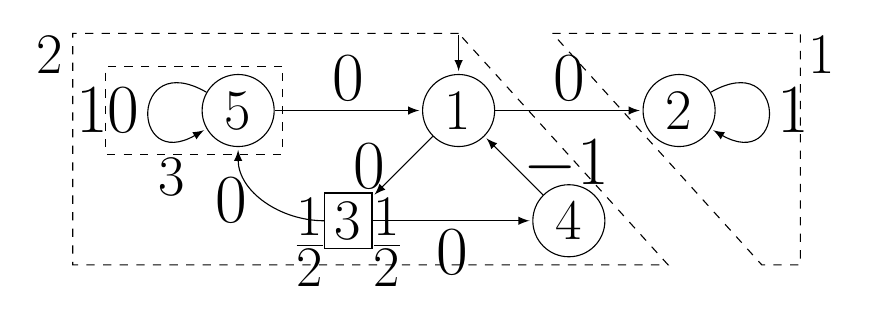
\begin{tikzpicture}[->,>=latex,shorten >=1pt,auto,node
    distance=2.5cm,bend angle=45,font=\Huge,scale=0.7]
    \tikzstyle{p1}=[draw,circle,text centered,minimum size=6mm]
    \tikzstyle{p2}=[draw,rectangle,text centered,minimum size=6mm]
    \tikzstyle{empty}=[]
    \node[p1] (1) at (0,0) {$\state_{1}$};
    \node[p1] (2) at (4,0) {$\state_{2}$};
    \node[p2] (3) at (-2,-2) {$\state_{3}$};
    \node[p1] (4) at (2,-2) {$\state_{4}$};
    \node[p1] (5) at (-4,0) {$\state_{5}$};
    \node[empty] (ec1) at (-5.2, -1.2) {$\ec_{3}$};
    \node[empty] (ec2) at (-7.4, 1) {$\ec_{2}$};
    \node[empty] (ec2) at (6.6, 1) {$\ec_{1}$};
    \node[empty] (proba1) at (-2.7, -2.4) {$\frac{1}{2}$};
    \node[empty] (proba2) at (-1.3, -2.4) {$\frac{1}{2}$};
    \coordinate[shift={(0mm,5mm)}] (init) at (1.north);
    \path
    (1) edge node[above] {$0$} (2)
    (5) edge node[above] {$0$} (1)
    (1) edge node[left,xshift=-1mm] {$0$} (3)
    (4) edge node[right] {$-1$} (1)
    (3) edge node[below] {$0$} (4)
    (init) edge (1)
    (5) edge [loop left, out=150, in=210,looseness=3, distance=16mm] node [left] {$10$} (5)
    (2) edge [loop right, out=30, in=330,looseness=3, distance=16mm] node [right] {$1$} (2)
    ;
	\draw[->,>=latex] (3) to[out=180,in=270] node[left,xshift=-1mm] {$0$} (5);
	\draw[dashed,-] (-3.2,0.8) -- (-6.4,0.8) -- (-6.4,-0.8) -- (-3.2,-0.8) -- (-3.2,0.8);
	\draw[dashed,-] (0,1.4) -- (-7,1.4) -- (-7,-2.8) -- (3.8,-2.8) -- (0,1.4);
	\draw[dashed,-] (1.7,1.4) -- (6.2,1.4) -- (6.2,-2.8) -- (5.5,-2.8) -- (1.7,1.4);
      \end{tikzpicture}}
      \caption{EC $\ec_{2}$ is losing. The set of MWECs is $\maxWinningECs = \winningECs = \{\ec_{1}, \ec_{3}\}$.}
\label{12-fig:bwcWinningECsComputationExample}
  \end{figure}

\begin{example}
Note that an EC is winning if $\playerOne$ has a worst-case winning strategy from \textit{all} vertices. This point is important as it may well be the case that winning strategies exist in a strict subset of vertices of the EC. This does not contradict the definition of ECs as strongly connected subgraphs, as the latter only guarantees that every vertex can be reached \textit{with probability one}, and not necessarily \textit{surely}. Hence one cannot call upon the prefix independence of the mean-payoff to extend the existence of a winning strategy to all vertices.

Such a situation can be observed on the arena of~\cref{12-fig:bwcWinningECsComputationExample}, where the EC~$\ec_{2}$ is losing (because from $\state_{1}$, the play $(\state_{1}\state_{3}\state_{4})^{\omega}$ can be forced by $\playerTwo$, yielding mean-payoff $-1/3 \leq 0$), while its sub-EC~$\ec_{3}$ is winning. From $\state_{1}$, $\playerOne$ can ensure to reach $\ec_{3}$ "almost-surely", but not "surely", which is critical in this case.
\end{example}


\subsection*{Maximal winning end-components} Based on these definitions, observe that~\cref{12-algo:BWC} does not actually compute the set $\winningECs$ containing all WECs, but rather the set $\maxWinningECs \subseteq \winningECs$, defined as $\maxWinningECs = \{\ec \in \winningECs \mid \forall\, \ec' \in \winningECs,\, \ec \subseteq \ec' \Rightarrow \ec = \ec'\}$, i.e., the set of \textit{maximal} WECs (MWECs).

The intuition on \textit{why we can} restrict our study to this subset is as follows. If an EC $\ec_{1} \in \winningECs$ is included in another EC $\ec_{2} \in \winningECs$, i.e., $\ec_{1} \subseteq \ec_{2}$, we have that the maximal expected value achievable in $\ec_{2}$ is at least equal to the one achievable in~$\ec_{1}$. Indeed, $\playerOne$ can reach $\ec_{1}$ with probability one (by virtue of $\ec_{2}$ being an EC and $\ec_{1} \subseteq \ec_{2}$) and stay in it forever with probability one (by virtue of $\ec_{1}$ being an EC): hence the expectation of such a strategy would be equal to what can be obtained in~$\ec_{1}$ thanks to the prefix independence of the mean-payoff. This property implies that it is sufficient to consider MWECs in our computations.

As for \textit{why we do it}, observe that the complexity gain is critical. The number of WECs can be as large as~$\vert\winningECs\vert \leq \vert\ecsSet\vert \leq 2^{\vert V\vert}$, that is, exponential in the size of the input. Yet, the number of MWECs is bounded by $\vert\maxWinningECs\vert \leq \vert V\vert$ as they are disjoint by definition: for any two WECs with a non-empty intersection, their union also constitutes an EC, and is still winning because $\playerOne$ can essentially stick to the EC of her choice.

The computation of the set $\maxWinningECs$ is executed by a recursive subalgorithm calling polynomially-many times an oracle solving the worst-case problem (e.g., following the pseudo-polynomial-time algorithm of~\cref{chap:payoffs}). \todo{I need a label on Subsect. 4.3.4 to cite it precisely.} Roughly sketched, this algorithm computes the maximal EC decomposition of an MDP (in polynomial time by~\cref{5-thm:MEC-decomposition-complexity}), then checks for each EC $\ec$ in the decomposition (their number is polynomial) if $\ec$ is winning or not, which requires a call to an oracle solving the worst-case threshold problem on the corresponding subgame. If $\ec$ is losing, it may still be the case that a sub-EC $\ec' \subsetneq \ec$ is winning. Therefore we recurse on the MDP reduced to $\ec$, where vertices from which $\playerTwo$ can win in $\ec$ have been removed (they are a no-go for $\playerOne$). Hence the stack of calls is also at most polynomial.

\begin{lemma}
\label{12-lem:MWEC}
The set $\maxWinningECs$ of MWECs can be computed in pseudo-polynomial time, and deciding if a set of vertices $U \subseteq V$ belongs to $\maxWinningECs$ is in $\NP \cap \coNP$.
\end{lemma}

The complexity follows from~\cref{4-thm:MP-NPcoNP} and $\P^{\NP \cap \coNP} = \NP \cap \coNP$~\cite{Brassard:1979}.

\begin{example}
Consider the running example in~\cref{12-fig:bwcRunningExample}. Note that vertices $\state_{1}$, $\state_{2}$ and $\state_{5}$ do not belong to any EC: given any strategy of $\playerOne$ in $\markovProcess$, with probability one, any consistent play will only visit these vertices a finite number of times (\cref{5-lem:EC-inf}). The set of \textit{MWECs} is $\maxWinningECs = \{\ec_{2}, \ec_{3}\}$. Obviously, these ECs are disjoint. The set of WECs is larger, $\winningECs = \maxWinningECs \cup \{\{\state_{9}, \state_{10}\}, \{\state_{6}, \state_{7}\}\}$.

End-component $\ec_{1}$ is \textit{losing}: in the subarena $\gameNonZero \reduc \ec_{1}$, Adam's strategy consisting in always picking the $-1$ edge guarantees a negative mean-payoff. Note that this edge is present in $\edgesNonZero$ as it is assigned probability $1/2$ by the stochastic model $\stratStoch$. Here, we witness why it is important to base our definition of WECs on $\gameNonZero$ rather than $\arena$. Indeed, in $\arena \reduc \ec_{2}$, it is also possible for $\playerTwo$ to guarantee a negative mean-payoff by always choosing edges with weight $-1$. However, to achieve this, $\playerTwo$ has to pick edges that are \textit{not} in $\edgesNonZero$: this will never happen against the stochastic model and as such, this can be watched by $\playerOne$ to see if $\playerTwo$ uses an arbitrary antagonistic strategy, and dealt with. If $\playerTwo$ conforms to $\edgesNonZero$, i.e., if he plays in $\gameNonZero$, he has to pick the edge of weight $1$ in $\state_{7}$ and $\playerOne$ has a worst-case winning strategy consisting in always choosing to go in $\state_{7}$. This EC is thus classified as \textit{winning}. Note that for $\ec_{3}$, in both subarenas $\arena \reduc \ec_{3}$ and $\gameNonZero \reduc \ec_{3}$, $\playerOne$ can guarantee a strictly positive mean-payoff by playing $(\state_{9}\,\state_{10})^\omega$: even \textit{arbitrary} strategies of $\playerTwo$ cannot endanger $\playerOne$ in this case.

Lastly, consider the arena depicted in~\cref{12-fig:bwcWinningECsComputationExample}. While $\ec_{2}$ is a strict superset of $\ec_{3}$, the former is losing whereas the latter is winning, as explained above. Hence, the set $\maxWinningECs$ is equal to $\{\ec_{1}, \ec_{3}\}$.
\end{example}

\subsection*{Ensure reaching winning end-components} As discussed, under any arbitrary strategy of $\playerOne$, vertices visited infinitely often form an EC with probability one (\cref{5-lem:EC-inf}). Now, if we take a \textit{finite-memory} strategy that \textit{satisfies} the $\BWC$ problem, we can refine this result and state that they form a \textit{winning} EC with probability one. Equivalently, let $\infVisited{\play}$ denote the set of vertices visited infinitely often along a play $\play$: we have that the probability that a play~$\play$ is such that $\infVisited{\play} = \ec$ for some $\ec \in \ecsSet \setminus \winningECs$ is zero. The equality is crucial. It may be the case, with non-zero probability, that $\infVisited{\play} = \ec' \subsetneq \ec$, for some $\ec' \in \winningECs$, and $\ec \in \ecsSet \setminus \winningECs$ (hence the recursive algorithm to compute $\maxWinningECs$). It is clear that~$\playerOne$ should not visit all the vertices of a LEC forever, as then she would not be able to guarantee the worst-case threshold inside the corresponding subarena.\footnote{This is no longer true if Eve may use infinite memory: there may still be some incentive to stay in a LEC. But this goes beyond the scope of our overview.}

\begin{lemma}
\label{12-lem:EC-inf}
For any initial vertex $ v_0 $ and finite-memory strategy $ \sigma $ that satisfies the BWC problem, it holds that $ \probm^\sigma_{\markovProcess, v_0} ( \{\play \mid \infVisited{\play} \in \winningECs \}) = 1 $. 
\end{lemma}

We denote $\negligibleStates = V \setminus \bigcup_{\ec \in \maxWinningECs} \ec$ the set of vertices that, with probability one, are only seen a finite number of times when a $\BWC$ satisfying strategy is played, and call them \textit{negligible} vertices.

Our ultimate goal here is to modify the colouring of $\markovProcess$ from $c$ to $c'$, such that a classical optimal strategy for the expected value problem (\cref{5-thm:general-mp-main}) using this new colouring $c'$ will naturally avoid LECs and prescribe which WECs are the most interesting to reach for a $\BWC$ strategy on the initial arena $\arena$ and MDP $\markovProcess$ with colouring $c$. For the sake of readability, let us simply use $\markovProcess$ and $\markovProcess'$ to refer to MDP $\markovProcess$ with respective colourings $c$ and $c'$.

Observe that the expected value obtained in $\markovProcess$ by any $\BWC$ satisfying strategy of $\playerOne$ only depends on the weights of edges involved in WECs, or equivalently, in MWECs (as the set of plays that are not trapped in them has measure zero). Consequently, we define colouring $c'$ as follows: we keep the weights unchanged in edges that belong to some $\ec \in \maxWinningECs$, and we put them to zero everywhere else, i.e., on any edge involving a negligible vertex. Weight zero is taken because it is lower than the expectation granted by WECs, which is \textit{strictly} greater than zero by definition (as $\alpha = 0$).

\begin{example}
Consider $\ec_{1}$ in~\cref{12-fig:bwcRunningExample}. This EC is losing as argued before. The optimal expectation achievable in $\markovProcess \reduc \ec_{1}$ by $\playerOne$ is $4$: this is higher than what is achievable in both $\ec_{2}$ and $\ec_{3}$. Note that there exists no WEC included in $\ec_{1}$. By~\cref{chap:mdp}, we know that any strategy of $\playerOne$ will see its expectation bounded by the maximum between the optimal expectations of the ECs $\ec_{1}$, $\ec_{2}$ and $\ec_{3}$. Our previous arguments further refine this bound by restricting it to the maximum between the expectations of $\ec_{2}$ and $\ec_{3}$. Indeed, $\playerOne$ cannot benefit from the expected value of $\ec_{1}$ while using finite memory, as being trapped in~$\ec_{1}$ induces the existence of plays losing for the worst-case. Hence there is no point in playing inside $\ec_{1}$ and $\playerOne$ may as well cross it directly and try to maximize its expectation using the WECs, $\ec_{2}$ and $\ec_{3}$. The set of negligible vertices in $\markovProcess$ is $\negligibleStates = V \setminus (\ec_{2} \cup \ec_{3}) = \{\state_{1}, \state_{2}, \state_{3}, \state_{4}, \state_{5}\}$. We depict $\markovProcess'$ in~\cref{12-fig:bwc_mp_modifiedMDP}.

In the arena depicted in~\cref{12-fig:bwcWinningECsComputationExample}, we already observed that $\ecsSet = \{\ec_{1}, \ec_{2}, \ec_{3}\}$ and $\winningECs = \maxWinningECs = \{\ec_{1}, \ec_{3}\}$. Consider the negligible vertex $\state_{1} \in \negligibleStates = \ec_{2} \setminus \ec_{3}$. A finite-memory strategy of $\playerOne$ may only take the edge $(\state_{1}, \state_{3})$ finitely often in order to ensure the worst-case requirement. If $\playerOne$ were to play this edge repeatedly, the losing play $(\state_{1}\state_{3}\state_{4})^{\omega}$ would exist (while of probability zero). Therefore, $\playerOne$ can only ensure that $\ec_{3}$ is reached with a probability arbitrarily close to one, and not equal to one, because at some point, she has to switch to edge $(\state_{1}, \state_{2})$ (after a bounded time since $\playerOne$ uses a finite-memory strategy).
\end{example}

\begin{figure}[htb]
  \centering   
  \scalebox{0.8}{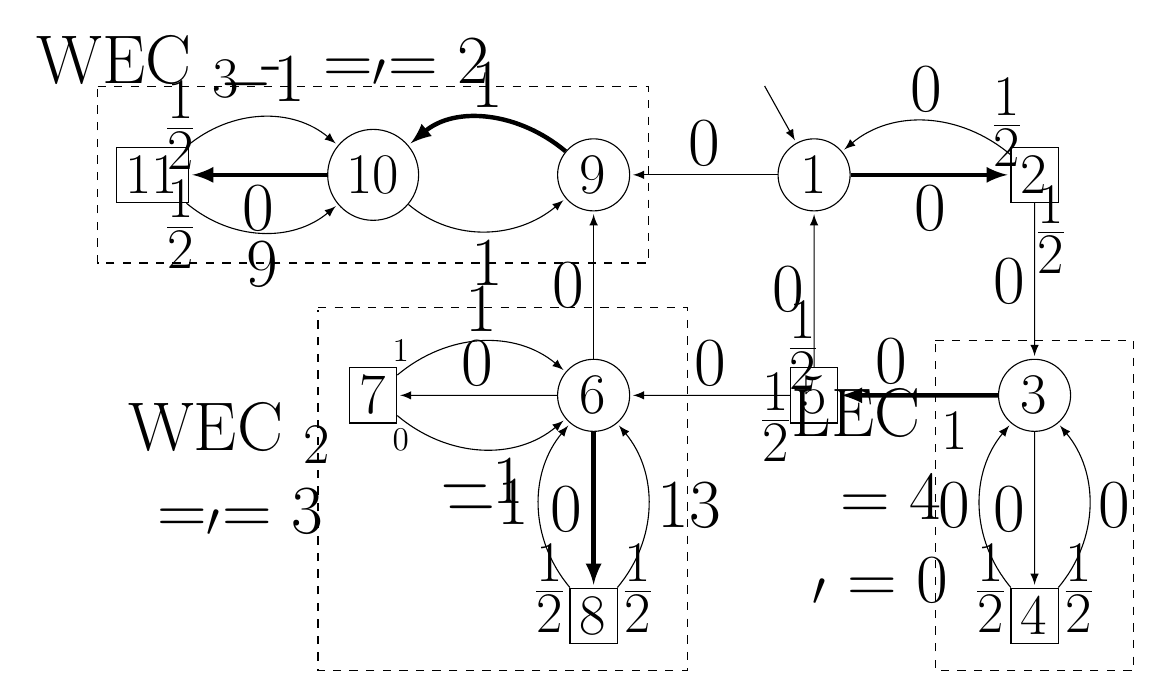
\begin{tikzpicture}[->,>=latex,shorten >=1pt,auto,node
    distance=2.5cm,bend angle=45,font=\Huge,scale=0.7]
    \tikzstyle{p1}=[draw,circle,text centered,minimum size=6mm]
    \tikzstyle{p2}=[draw,rectangle,text centered,minimum size=6mm]
    \tikzstyle{empty}=[]
    \node[p1] (1) at (0,0) {$\state_{9}$};
    \node[p1] (2) at (4,0) {$\state_{1}$};
    \node[p2] (3) at (8,0) {$\state_{2}$};
    \node[p1] (4) at (8,-4) {$\state_{3}$};
    \node[p2] (5) at (8,-8) {$\state_{4}$};
    \node[p2] (6) at (4,-4) {$\state_{5}$};
    \node[p1] (7) at (0,-4) {$\state_{6}$};
    \node[p2] (8) at (-4,-4) {$\state_{7}$};
    \node[p1] (9) at (-4,0) {$\state_{10}$};
    \node[p2] (10) at (-8,0) {$\state_{11}$};
    \node[p2] (11) at (0,-8) {$\state_{8}$};
    \node[empty] (swec) at (-6, 1.9) {WEC $\ec_{3}$ - $\expv_{\markovProcess} = \expv_{\markovProcess'} = 2$};
    \node[empty,align=center] (wwec) at (-6.6, -5.5) {WEC $\ec_{2}$\\$\expv_{\markovProcess} = \expv_{\markovProcess'} = 3$};
    \node[empty,align=center] (lec) at (5.2, -6) {LEC $\ec_{1}$\\$\expv_{\markovProcess} = 4$\\$\expv_{\markovProcess'}  = 0$};
    \node[empty] (proba5a) at (7.2, -7.5) {$\frac{1}{2}$};
    \node[empty] (proba5b) at (8.8, -7.5) {$\frac{1}{2}$};
    \node[empty] (proba3a) at (8.3, -1) {$\frac{1}{2}$};
    \node[empty] (proba3b) at (7.5, 0.95) {$\frac{1}{2}$};
    \node[empty] (proba8a) at (-3.5, -3.2) {{\large $1$}};
    \node[empty] (proba8b) at (-3.5, -4.8) {{\large $0$}};
    \node[empty] (proba10a) at (-7.5, 0.9) {$\frac{1}{2}$};
    \node[empty] (proba10b) at (-7.5, -0.9) {$\frac{1}{2}$};
    \node[empty] (proba11a) at (0.8, -7.5) {$\frac{1}{2}$};
    \node[empty] (proba11b) at (-0.8, -7.5) {$\frac{1}{2}$};
    \node[empty] (proba6a) at (3.8, -3.1) {$\frac{1}{2}$};
    \node[empty] (proba6b) at (3.3, -4.4) {$\frac{1}{2}$};
    \coordinate[shift={(-3mm,8mm)}] (init) at (2.north west);
    \path
    (2) edge node[above] {$0$} (1)
    (6) edge node[above] {$0$} (7)
    (4) edge[ultra thick] node[above left] {$0$} (6)
    (3) edge node[left] {$0$} (4)
    (6) edge node[left] {$0$} (2)
    (4) edge node[left] {$0$} (5)
    (7) edge node[above] {$0$} (8)
    (7) edge node[left] {$0$} (1)
    (init) edge (2)
    ;
	\draw[->,>=latex] (3) to[out=140,in=40] node[above] {$0$} (2);
	\draw[->,>=latex,ultra thick] (2) to[out=0,in=180] node[below] {$0$} (3);
	\draw[->,>=latex] (5) to[out=50,in=310] node[right] {$0$} (4);
	\draw[->,>=latex] (5) to[out=130,in=230] node[left] {$0$} (4);
	\draw[->,>=latex] (8) to[out=40,in=140] node[above] {$1$} (7);
	\draw[->,>=latex] (8) to[out=320,in=220] node[below] {$-1$} (7);
	\draw[->,>=latex,ultra thick] (1) to[out=140,in=40] node[above] {$1$} (9);
	\draw[->,>=latex] (9) to[out=320,in=220] node[below] {$1$} (1);
	\draw[->,>=latex,ultra thick] (9) to[out=180,in=0] node[below] {$0$} (10);
	\draw[->,>=latex] (10) to[out=40,in=140] node[above] {$-1$} (9);
	\draw[->,>=latex] (10) to[out=320,in=220] node[below] {$9$} (9);
	\draw[->,>=latex,ultra thick] (7) to[out=270,in=90] node[left] {$0$} (11);
	\draw[->,>=latex] (11) to[out=130,in=230] node[left] {$-1$} (7);
	\draw[->,>=latex] (11) to[out=50,in=310] node[right] {$13$} (7);
	\draw[dashed,-] (-9,1.6) -- (1,1.6) -- (1,-1.6) -- (-9,-1.6) -- (-9,1.6);
	\draw[dashed,-] (6.2,-3) -- (9.8,-3) -- (9.8,-9) -- (6.2,-9) -- (6.2,-3);
	\draw[dashed,-] (-5,-2.4) -- (1.7,-2.4) -- (1.7,-9) -- (-5,-9) -- (-5,-2.4);
      \end{tikzpicture}}
      \caption{Putting all weights outside MWECs to zero naturally drives the optimal expectation strategy in $\markovProcess'$, depicted by the thick edges, toward the highest valued MWECs. ECs are annotated with their corresponding optimal expectations in the original MDP $\markovProcess$ and the modified MDP $\markovProcess'$.}
\label{12-fig:bwc_mp_modifiedMDP}
  \end{figure}

\subsection*{Reach the highest valued winning end-components} We compute the maximal expected mean-payoff $\beta^{\ast}$ that can be achieved by $\playerOne$ in $\markovProcess'$, from $v_0$. This computation takes polynomial time and memoryless strategies suffice to achieve the maximal value, as established in~\cref{5-thm:general-mp-main}.

As discussed before, such a strategy reaches an EC of $\markovProcess'$ with probability one. Basically, we build a strategy that favours reaching ECs with high associated expectations in $\markovProcess'$.

We argue that the ECs reached with probability one by this strategy are necessarily WECs in $\markovProcess$. Clearly, if a WEC is reachable instead of a losing one, it will be favoured because of the weights definition in $\markovProcess'$ (expectation is strictly higher in WECs). Thus it remains to check if the set of WECs is reachable with probability one from any vertex in $V$. That is the case because of the preprocessing: we know that all vertices are winning for the worst-case requirement. Clearly, from any vertex in $A = V \setminus \bigcup_{\ec \in \ecsSet} \ec$, $\playerOne$ cannot ensure to stay in $A$ (otherwise it would form an EC) and thus must be able to win the worst-case requirement from reached ECs. Now for any vertex in $B = \bigcup_{\ec \in \ecsSet} \ec \setminus \bigcup_{\ec \in \maxWinningECs} \ec$, i.e., vertices in LECs and not in any sub-EC winning, $\playerOne$ cannot win the worst-case by staying in $B$, by definition of LEC. Since we know $\playerOne$ can ensure the worst-case by hypothesis, it is clear that she must be able to reach $C = \bigcup_{\ec \in \maxWinningECs} \ec$ from any vertex in $B$, as claimed.

\subsection*{Inside winning end-components} Based on that, we know that WECs of $\markovProcess$ will be reached with probability one when maximizing the expected value in $\markovProcess'$. Let us first consider what we can say about such ECs if we assume that $\edgesNonZero = \edges$, i.e., if the stochastic model $\stratStoch$ maps all possible edges to non-zero probabilities. 
We establish a finite-memory \textit{combined strategy} $\stratComb$ of $\playerOne$ that ensures~(i) worst-case satisfaction while yielding (ii) an expected value $\varepsilon$-close to the maximal expectation inside the EC.

For two well-chosen parameters $\stepsExp, \stepsWC \in \N$, it is informally defined as follows: in phase $\typeA$, play a memoryless expected value optimal strategy $\stratExp$ for $\stepsExp$ steps and memorize $\cmbSum \in \Z$, the sum of weights along these steps; in phase $\typeB$, if $\cmbSum > 0$, go to~$\typeA$, otherwise play a memoryless worst-case optimal strategy $\stratWC$ for~$\stepsWC$ steps, then go to $\typeA$. In $\typeA$, $\playerOne$ tries to increase her expectation and approach the optimal one, while in $\typeB$, she compensates, if needed, losses that occurred in $\typeA$.

The two memoryless strategies exist on the subarena induced by the EC: by definition of ECs, based on~$\edgesNonZero$, the stochastic model of $\playerTwo$ will never be able to force leaving the EC against the combined strategy.

A key result to our approach is the existence of values for $\stepsExp$ and~$\stepsWC$ such that~(i) and (ii) are verified. We see plays as sequences of periods, each starting with phase~$\typeA$.

First, for any $\stepsExp$, it is possible to define $\stepsWC(\stepsExp)$ such that any period composed of phases~$\typeA+\typeB$ ensures a mean-payoff at least $1/(\stepsExp+\stepsWC) > 0$. Periods containing only phase $\typeA$ trivially induce a mean-payoff at least~$1/\stepsExp$ as they are not followed by phase $\typeB$. Both rely on the weights being integers. As the length of any period is bounded by $(\stepsExp+\stepsWC)$, the inequality remains strict for the mean-payoff of any play, granting~(i).

Now, consider parameter $\stepsExp$. Clearly, when~$\stepsExp \rightarrow \infty$, the expectation over phase $\typeA$ tends to the optimal one. Nevertheless, phases~$\typeB$ also contribute to the overall expectation of the combined strategy, and (in general) lower it so that it is strictly less than the optimal for any $\stepsExp, \stepsWC \in \N$. Hence to prove (ii), we not only need that the probability of playing phase $\typeB$ decreases when $\stepsExp$ increases, but also that it decreases faster than the increase of $\stepsWC$, needed to ensure~(i), so that overall, the contribution of phases~$\typeB$ tends to zero when $\stepsExp \rightarrow \infty$. This is indeed the case and is proved using results bounding the probability of observing a mean-payoff significantly (more than some $\varepsilon$) different than the optimal expectation along a phase $\typeA$ of length $\stepsExp \in \N$: this probability decreases exponentially when~$\stepsExp$ increases, while $\stepsWC$ only needs to be polynomial in $\stepsExp$.

\begin{theorem}
\label{12-thm:insideWinning}
Let $U \in \winningECs$ be a WEC, $\stratStoch$ be such that $\edgesNonZero = \edges$, $v_0 \in U$ be the initial vertex, and let $\beta^\ast \in \Q$ be the maximal expected value achievable by $\playerOne$ in EC $U$. Then, for all~$\varepsilon > 0$, there exists a finite-memory strategy of $\playerOne$ that satisfies the $\BWC$ problem for the thresholds pair $(0,\, \beta^\ast - \varepsilon)$.
\end{theorem}

\begin{example}
Consider the subarena $\gameNonZero \reduc \ec_{3} = \arena \reduc \ec_{3}$ from~\cref{12-fig:bwcRunningExample} and the initial vertex $\state_{10}$. Clearly, the worst-case requirement can be satisfied, that is why the EC is classified as winning. Always choosing to go to~$\state_{9}$ when in $\state_{10}$ is an optimal memoryless worst-case strategy $\stratWC$ that guarantees a mean-payoff $\alpha^\ast = 1$. Its expectation is $\expv^{\stratWC}_{(\arena \reduc \ec_{3})_{\tau^\text{stoch}},v_{10}}[\MeanPayoff^{-}] = 1$. On the other hand, the strategy $\stratExp$ that always selects the edge going to $\state_{11}$ is optimal regarding the expected value criterion: it induces expectation $\beta^\ast = \big(0 + \big(1/2 \cdot 9 + 1/2 \cdot (-1)\big)\big)/2 = 2$ against the stochastic model $\stratStoch$. However, it can only guarantee a mean-payoff of value $-1/2$ in the worst-case.

By the reasoning above, we know that it is possible to find finite-memory strategies satisfying the $\BWC$ problem for any thresholds pair $(0,\, 2 - \varepsilon)$, $\varepsilon > 0$. In particular, consider the thresholds pair $(0,\, 3/2)$. We build a combined strategy~$\stratComb$ as sketched before. Let $\stepsExp = \stepsWC = 2$: the strategy plays the edge $(\state_{10}, \state_{11})$ once, then if the edge of value $9$ has been chosen by $\playerTwo$, it chooses $(\state_{10}, \state_{11})$ again; otherwise it chooses the edge $(\state_{10}, \state_{9})$ once and then resumes choosing $(\state_{10}, \state_{11})$. This strategy satisfies the $\BWC$ problem. In the worst-case,~$\playerTwo$ always chooses the $-1$ edge, but each time he does so, the $-1$ is followed by two~$+1$ thanks to the cycle $\state_{10} \state_{9} \state_{10}$. Strategy $\stratComb$ hence guarantees a mean-payoff equal to $(0 - 1 + 1 + 1)/4 = 1/4 > 0$ in the worst-case. For the expected value requirement, we can build the induced Markov chain $(\arena \reduc \ec_{3})_{\stratComb, \tau^\text{stoch}}$ (\cref{12-fig:mp_insideSWEC_MC}) and check that its expectation is $\expv^{\stratComb}_{(\arena \reduc \ec_{3})_{\tau^\text{stoch}},v_{10}}[\MeanPayoff^{-}] = 5/3 > 3/2$ (\cref{chap:payoffs}).

\begin{figure}[ht]
  \centering 
  \scalebox{0.8}{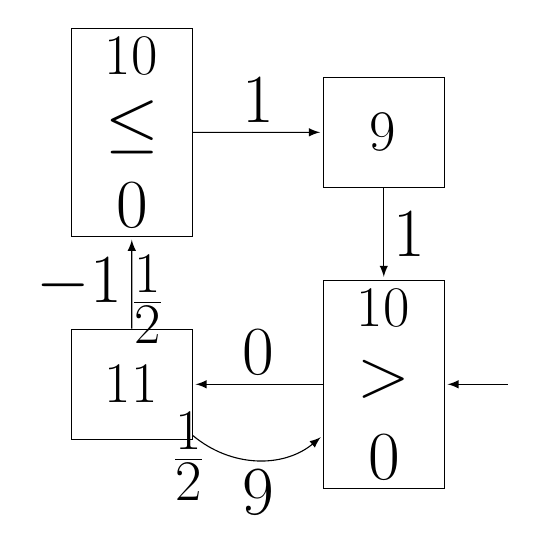
\begin{tikzpicture}[->,>=latex,shorten >=1pt,auto,node
    distance=2.5cm,bend angle=45,font=\Huge,scale=0.8]
    \tikzstyle{p1}=[draw,circle,text centered,minimum size=6mm]
    \tikzstyle{p2}=[draw,rectangle,text centered,minimum size=14mm,text width=13mm]
    \tikzstyle{p3}=[draw,diamond,text centered,minimum size=20mm,text width=13mm]
    \tikzstyle{empty}=[]
    \node[p2] (1) at (0,0) {$\state_{10}$\\$\cmbSum > 0$};
    \node[p2] (2) at (-4,0) {$\state_{11}$};
    \node[p2] (3) at (-4,4) {$\state_{10}$\\$\cmbSum \leq 0$};
    \node[p2] (4) at (0,4) {$\state_{9}$};
    \node[empty] (a) at (-3.75, 1.35) {$\frac{1}{2}$};
    \node[empty] (b) at (-3.10, -1.15) {$\frac{1}{2}$};
    \coordinate[shift={(8mm,0mm)}] (init) at (1.east);
    \path
    (1) edge node[above] {$0$} (2)
    (2) edge node[left] {$-1$} (3)
    (3) edge node[above] {$1$} (4)
    (4) edge node[right] {$1$} (1)
    (init) edge (1)
    ;
	\draw[->,>=latex] (2) to[out=320,in=220] node[below] {$9$} (1);
      \end{tikzpicture}}
      \caption{Markov chain induced by the combined strategy $\stratComb$ and the stochastic model $\stratStoch$ over the WEC $\ec_{3}$ of $\arena$.}
\label{12-fig:mp_insideSWEC_MC}
\end{figure}
\end{example}

\begin{remark}
\label{12-rmk:bwcMemorylessNotEnough}
Memoryless strategies do not suffice for the $\BWC$ problem, even with randomization. Indeed, the edge $(\state_{10}, \state_{11})$ cannot be assigned a non-zero probability as it would endanger the worst-case requirement (since the play~$(\state_{10}\state_{11})^{\omega}$ cycling on the edge of weight $-1$ would exist and have a negative mean-payoff). Hence, the only acceptable memoryless strategy is $\stratWC$, which has only an expectation of $1$.
\end{remark}


Now, consider what happens if $\edgesNonZero \subsetneq E$. Then, if $\playerTwo$ uses an arbitrary strategy, he can take edges of probability zero, i.e., in $E \setminus \edgesNonZero$, either staying in the EC, or leaving it. In both cases, this must be taken into account in order to satisfy the worst-case constraint as it may involve dangerous weights (recall that zero-probability edges are not considered when an EC is classified as winning or not). Fortunately, if this were to occur, $\playerOne$ could switch to a worst-case winning memoryless strategy $\stratSecure$, which exists in all vertices thanks to the preprocessing, to preserve the worst-case requirement. Regarding the expected value, this has no impact as it occurs with probability zero against $\stratStoch$. The strategy to follow in WECs hence adds this reaction procedure to the combined strategy: we call it the \textit{witness-and-secure strategy} $\stratWNS$.

\begin{theorem}
\label{12-thm:wns}
Let $U \in \winningECs$ be a WEC, $v_0 \in U$ be the initial vertex, and $\beta^\ast \in \Q$ be the maximal expected value achievable by $\playerOne$ in EC $U$. Then, for all~$\varepsilon > 0$, there exists a finite-memory strategy of $\playerOne$ that satisfies the $\BWC$ problem for the thresholds pair $(0,\, \beta^\ast - \varepsilon)$.
\end{theorem}

\begin{example}
Consider the WEC $\ec_{2}$ in~\cref{12-fig:bwcRunningExample} and the initial vertex $\state_{6} \in \ec_{2}$. $\playerOne$ can ensure a strictly positive mean-payoff in the subarena $\gameNonZero \reduc \ec_{2}$, but not in $\arena \reduc \ec_{2}$. Indeed, it is easy to see that by always choosing the $-1$ edges (which requires an edge $(\state_{7}, \state_{6}) \in \edgesNonZero \setminus \edges$), $\playerTwo$ can ensure a negative mean-payoff whatever the strategy of $\playerOne$. However, there exists a strategy that ensures the worst-case constraint, i.e., that yields a strictly positive mean-payoff against any strategy of Adam, by leaving the EC. Let $\stratSecure$ be the memoryless strategy that takes the edge $(\state_{6}, \state_{9})$ and then cycle on $(\state_{10}\state_{9})^{\omega}$ forever: it guarantees a mean-payoff of $1 > 0$.

For a moment, consider the EC $\ec_{2}$ in $\gameNonZero$. Graphically, it means that the $-1$ edge from $\state_{7}$ to $\state_{6}$ disappears. In the subarena $\gameNonZero \reduc \ec_{2}$, there are two particular memoryless strategies. The optimal worst-case strategy $\stratWC$ guarantees a mean-payoff of $1/2 > 0$ by choosing to go to $\state_{7}$. The optimal expectation strategy $\stratExp$ yields an expected mean-payoff of $3$ by choosing to go to $\state_{8}$ (naturally this strategy yields the same expectation whether we consider edges in $\edgesNonZero$ or in $E$). Based on them, we build the combined strategy $\stratComb$ of Eve as defined earlier and by~\cref{12-thm:insideWinning}, for any $\varepsilon > 0$, there are values of $\stepsExp$ and $\stepsWC$ such that it satisfies the $\BWC$ problem for thresholds $(0,\, 3-\varepsilon)$ in $\gameNonZero \reduc \ec_{2}$. For instance, for $\stepsExp = \stepsWC = 2$, we have $\expv^{\stratComb}_{(\arena \reduc \ec_{2})_{\tau^\text{stoch}},v_{6}}[\MeanPayoff^{-}] = 13/6$.

We construct the witness-and-secure strategy $\stratWNS$ based on $\stratComb$ and $\stratSecure$ as described above. In this case, that means playing as $\stratComb$ until the $-1$ edge from $\state_{7}$ to $\state_{6}$ is taken by $\playerTwo$. This strategy ensures a worst-case mean-payoff equal to $1 > 0$ thanks to $\stratSecure$ and yields expectation $\expv^{\stratWNS}_{(\arena \reduc \ec_{2})_{\tau^\text{stoch}},v_{6}}[\MeanPayoff^{-}] = 13/6$ for $\stepsExp = \stepsWC = 2$.

Finally, notice that securing the mean-payoff by switching to  $\stratSecure$ \textit{is needed} to satisfy the worst-case requirement if $\playerTwo$ plays in $\edges \setminus \edgesNonZero$. Also, observe that it is still necessary to alternate according to $\stratComb$ in $\gameNonZero \reduc \ec_{2}$ and that playing $\stratExp$ is not sufficient to ensure the worst-case (because $\playerOne$ has to deal with the $-1$ edge from $\state_{8}$ to $\state_{6}$ that remains in $\edgesNonZero$).
\end{example}


\subsection*{Global strategy synthesis} In summary, (a) LECs should be avoided and will be by a strategy that optimizes the expectation on the MDP~$\markovProcess'$; (b) in WECs, $\playerOne$ can obtain ($\varepsilon$-closely) the expectation of the EC \textit{and} ensure the worst-case threshold.

Hence, we finally compare the value $\thresholdExp^{\ast}$ computed by~\cref{12-algo:BWC} with the expected value threshold $\thresholdExp$: (i) if it is strictly higher, we conclude that there exists a finite-memory strategy satisfying the $\BWC$ problem, and (ii) if it is not, we conclude that there does not exist such a strategy.

To prove (i), we establish a finite-memory strategy in $\arena$, called \textit{global strategy} $\stratGlobal$, of $\playerOne$ that ensures a strictly positive mean-payoff against an antagonistic adversary, and ensures an expected mean-payoff $\varepsilon$-close to $\thresholdExp^{\ast}$ (hence, strictly greater than $\thresholdExp$) against the stochastic adversary modeled by $\stratStoch$ (i.e., in $\markovProcess$). The intuition is as follows. We play the memoryless optimal strategy of $\markovProcess'$ for a sufficiently long time, defined by a parameter $\stepsGlobal \in \N$, in order to be with probability close to one in a WEC (the convergence is exponential by results on absorption times in Markov chains). Then, if we are inside a WEC, we switch to the corresponding witness-and-secure strategy (there is a different one for each MWEC) which, as sketched in the previous paragraph, ensures the worst-case and the expectation thresholds. If we are not yet in a WEC, then we switch to a worst-case winning strategy, which always exists thanks to the preprocessing. Thus the mean-payoff of plays that do not reach WECs is strictly positive. Since in WECs we are $\varepsilon$-close to the maximal expected value of the EC, we can conclude that it is possible to play the optimal expectation strategy of $\markovProcess'$ for sufficiently long to obtain an overall expected value which is arbitrarily close to $\thresholdExp^{\ast}$, and still guarantee the worst-case threshold in all consistent plays.

To prove (ii), it suffices to understand that only ECs have an impact on the expectation, and that LECs cannot be used forever without endangering the worst-case requirement.

Note that given a winning strategy on $\arena$, it is possible to build a corresponding winning strategy on $\arena^{i}$ by reintegrating the memory states of $\tau^i$ in the memory structure of the winning strategy of $\playerOne$. Hence~\cref{12-algo:BWC} is correct and complete.

\begin{theorem}
\label{12-thm:bwcCorrectAndComplete}
If~\cref{12-algo:BWC} answers \textsc{Yes}, then there exist values of the parameters such that the pure finite-memory global strategy $\stratGlobal$ satisfies the $\BWC$ mean-payoff problem. In the opposite case, there exists no finite-memory strategy that satisfies the $\BWC$ mean-payoff problem.
\end{theorem}


\begin{example}
Consider the arena in~\cref{12-fig:bwcRunningExample} and the associated MDP $\markovProcess$. Following~\cref{chap:mdp}, analysis of the maximal ECs $\ec_{1}$, $\ec_{2}$ and $\ec_{3}$ reveals that the maximal expected mean-payoff achievable in $\markovProcess$ is $4$. It is for instance obtained by the memoryless strategy that chooses to go to $\state_{2}$ from $\state_{1}$ and to $\state_{4}$ from $\state_{3}$. Observe that playing in $\ec_{1}$ forever is needed to achieve this expectation. By~\cref{12-lem:EC-inf}, this should not be allowed as the worst-case cannot be ensured if it is. Indeed, $\playerTwo$ can produce worst-case losing plays by playing the $-1$ edge. Clearly, the maximal expected value that $\playerOne$ can ensure while guaranteeing the worst-case requirement is thus bounded by the maximal expectation in $\markovProcess'$, i.e., by $3$, as depicted in~\cref{12-fig:bwc_mp_modifiedMDP}. Let $\stratExp$ denote an optimal memoryless expectation strategy in $\markovProcess'$ that tries to enter~$\ec_{2}$ by playing $(\state_{1}, \state_{2})$ and $(\state_{3}, \state_{5})$, and then plays edge $(\state_{6}, \state_{8})$ forever (thick edges in~\cref{12-fig:bwc_mp_modifiedMDP}).



Observe that~\cref{12-algo:BWC} answers \textsc{Yes} for any thresholds pair $(0,\, \thresholdExp)$ such that $\thresholdExp < 3$. For the sake of illustration, we construct the global strategy~$\stratGlobal$ as presented earlier, with $\stepsGlobal = 6$ and $\stepsExp = \stepsWC = 2$. For the first six steps, it behaves exactly as $\stratExp$. Note that after the six steps, the probability of being in $\ec_{2}$ is $1/4 + 1/8 = 3/8$. Then, $\stratGlobal$ switches to another strategy depending on the current vertex ($\stratWNS$ or $\stratWC$) and sticks to this strategy forever. In particular, if the current vertex belongs to $\ec_{2}$, it switches to $\stratWNS$ for $\stepsExp = \stepsWC = 2$, which guarantees the worst-case threshold and induces an expectation of $13/6$. By definition of $\stratGlobal$, if the current vertex after six steps is not in $\ec_{2}$, then $\stratGlobal$ switches to $\stratWC$ which guarantees a mean-payoff of $1$ by reaching vertex $\state_{9}$ and then playing $(\state_{9}\state_{10})^{\omega}$. Overall, the expected mean-payoff of $\stratGlobal$ against $\stratStoch$ is
\begin{equation*}
\expv^{\stratGlobal}_{\arena_{\tau^\text{stoch}},v_{1}}[\MeanPayoff^{-}] \geq \dfrac{3}{8}\cdot\dfrac{13}{6} + \dfrac{5}{8}\cdot 1 = \dfrac{23}{16}.
\end{equation*}
Notice that by taking $\stepsGlobal$, $\stepsExp$ and $\stepsWC$ large enough, it is possible to satisfy the $\BWC$ problem for any $\thresholdExp < 3$ with the strategy $\stratGlobal$. Also, observe that the WEC~$\ec_{2}$ is crucial to achieve expectations strictly greater than $2$, which is the upper bound when limited to EC $\ec_{3}$. For instance, $\stepsGlobal = 25$ and $\stepsExp = \stepsWC = 2$ implies an expectation strictly greater than $2$ for the global strategy.

Lastly, note that in general, the maximal expectation achievable in $\markovProcess'$ (and thus in $\markovProcess$ when limited to strategies that respect the worst-case requirement) may depend on a combination of ECs instead of a unique one. This is transparent through the solving of the expected value problem in the MDP $\markovProcess'$. Hence, the approach followed by~\cref{12-algo:BWC} is a way of solving a complex problem by breaking it into smaller pieces.
\end{example}

\subsection*{Complexity bounds} The input size of the algorithm depends on the size of the arena, the size of the memory structure for the stochastic model, and the encodings of probabilities, weights and thresholds. We can prove that all computing steps require (deterministic) polynomial time except for calls to an algorithm solving the worst-case threshold problem, which is in $\NP \cap \coNP$ and not known to be in $\P$ (\cref{4-thm:MP-NPcoNP}). Hence, the overall complexity of the $\BWC$ problem is in $\NP \cap \coNP$ (using $\P^{\NP \cap \coNP} = \NP \cap \coNP$~\cite{Brassard:1979}) and may collapse to $\P$ if the worst-case problem were to be proved in $\P$.

The $\BWC$ problem is at least as difficult as the worst-case problem thanks to a trivial polynomial-time reduction from the latter to the former. Thus, membership to $\NP \cap \coNP$ can be seen as optimal regarding our current knowledge of mean-payoff games.

\begin{theorem}
\label{12-thm:bwcDecisionProblem}
The BWC mean-payoff problem is in $\NP \cap \coNP$ and at least as hard as solving mean-payoff games. Moreover, pseudo-polynomial-memory strategies may be necessary for Eve and are always sufficient.
\end{theorem}

The memory bounds follow from the (involved) probability results used to determine the values of parameters $K$, $L$ and $N$ in the aforementioned strategies: such parameters need to be polynomial in the size of the arena but also in the probabilities, weights and thresholds.

Using the pseudo-polynomial-time algorithm of~\cref{chap:payoffs} for mean-payoff games, \todo{I need label for Subsect. 4.3.4} we obtain the following corollary.

\begin{corollary}
\cref{12-algo:BWC} solves the BWC mean-payoff problem in pseudo-poly\-no\-mial time.
\end{corollary}

\subsection*{Wrap-up} As witnessed by our long overview, solving the beyond worst-case problem requires much more involved techniques than solving the two individual problems, worst-case and expected value, separately. Complexity-wise, it is fortunate that the problem stays in $\NP \cap \coNP$, and is no more complex that simple mean-payoff games. The multiobjective nature of the problem still incurs a cost with regard to strategies: whereas memoryless strategies suffice both in mean-payoff games and mean-payoff MDPs, we here need pseudo-polynomial memory. Finally, note that Eve does not need to use randomness: pure strategies still suffice.
